Ce chapitre présente le bloc qui permet au robot d'exploiter les moteurs et les encodeurs afin de se déplacer. Pour cela, ceux-ci doivent être configurés avant d'être utilisés respectivement comme actionneurs et capteurs dans une boucle fermée de régulation, afin d'obtenir une bonne précision et une résistance aux perturbations. Dans la section suivante, les moteurs et encodeurs ainsi que leur configuration sont brièvement présentés; la régulation sera ensuite couverte.\footnote{Ce chapitre couvre les fichiers \ilcode{wheels.*} et \ilcode{regul.*} du projet \ilcode{propulsion.X}}

\section{Moteurs et encodeurs}
\subsection{Commande en PWM des moteurs}
Les moteurs sont commandé en PWM. Comme le montre la figure \ref{fig:SignalServo}, les paramètres importants à ce bloc sont les suivants:
\begin{itemize}
  \item $\SI{3}{\milli\second} \leq T \leq \SI{20}{\milli\second}$
  \item $ \SI{1}{\milli\second} \leq T_{on} \leq \SI{2}{\milli\second}$
  \item $V_{mot}$ croît linéairement de $-V_{alim}$ à $+V_{alim}$ avec $T_{on}$
\end{itemize}
\begin{figure}[htbp]
\vspace{1.5em}
\centering
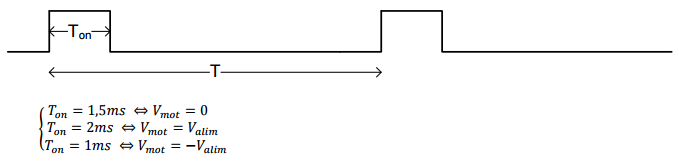
\includegraphics[width=0.85\textwidth,keepaspectratio]{SignalCommande.PNG}
\caption{\label{fig:SignalServo}Signal de commande des servomoteurs. [Source: \'Etude du déplacement du robot]}
\end{figure}

Le module output compare du microcontrôleur propulsion est donc utilisé pour générer la commande des moteurs. La configuration est opérée par la fonction \ilcode{configPWM}, qui initialise les paramètres suivants:
\begin{itemize}
  \item Output mapping des ports des output compare sur les pattes physiquement reliées aux moteurs
  \item Choix du mode de PWM: impulsion haute commençant au début de la période et de longueur variable, fixée par \ilcode{OCXRS}
  \item Choix du timer 2 comme valeur de comparaison
  \item Choix de $T_2 = \SI{10}{\milli\second}$, et démarrage du timer 2
\end{itemize}
Une fois $T_2$ fixé, il est plus facile de parler en terme de rapport cyclique qu'en longueur arbitraire. Puisque $T_2 = \SI{10}{\milli\second}$, on a directement:
\begin{align*}
  D = 0.1 &\Rightarrow V_{mot} = -V_{alim}\\
  D = 0.15 &\Rightarrow V_{mot} = 0\\
  D = 0.2 &\Rightarrow V_{mot} = +V_{alim}\\
\end{align*}
Le rapport cyclique est donc imposé par une simple instruction du type \ilcode{OCXRS = D*PR2}.

\begin{figure}[tbph]
\centering
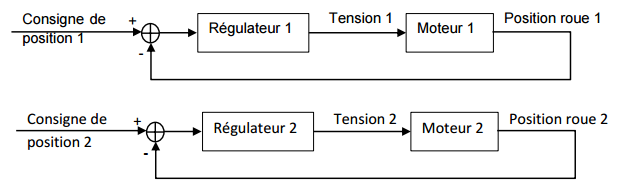
\includegraphics[width=0.85\textwidth,keepaspectratio]{BouclesdeRegul.PNG}
\caption{\label{fig:BouclesdeRegul}Schéma de Régulation}
\end{figure}

\subsection{Encodeurs en quadrature}
La rotation de chaque roue est mesurée par un encodeur en quadrature dont les paramètres importants sont les suivants:
\begin{itemize}
  \item 90 impulsions montantes par tour de roue
  \item Pas de détection d'un tour de roue complet
\end{itemize}
La sortie des encodeurs est traitée par le module QEI du microcontrôleur propulsion. Le module est configuré comme suit par la fonction \ilcode{configQEI}:
\begin{itemize}
  \item Input mapping des pattes physiquement reliées aux encodeurs sur les ports des QEI
  \item Choix du mode 4X sans index (pas disponible sur les encodeurs Vex): 360 impulsions par tour de roue
  \item Choix du maximum des compteurs à 360, et activation de l'interruption lorsqu'un compteur overflow, ce qui permet de reproduire le mécanisme d'index et de compter les tours de roues, afin de n'avoir virtuellement aucune limite sur les distances à mesurer (en cas d'utilisation prolongée, par exemple)
  \item \'Ecriture des routines d'overflow: \ilcode{xspins} est simplement incrémentée ou décrémentée en fonction de \ilcode{QEIxCON.UDPN}
\end{itemize}

\section{Implémentation du régulateur}

Une fois que notre robot est bien paramétré il doit être capable d'interpréter une consigne reçue et savoir quoi faire en fonction de la consigne. La partie concernant l'interprétation des ordres sera vue plus loin au chapitre 5.

Le rôle de cette sous-partie est d'expliquer les différents éléments du code de regul.c ainsi que de decision.c.

Notre robot peut suivre 3 états principaux :

\begin{itemize}
\item Straight
Le robot doit avancer en ligne droite sur une longueur bien définie.
\item Rotate
Le robot doit tourner d'un certain angle sur lui-même, la spécificité étant de tourner d'un côté ou de l'autre en fonction de l'importance de l'angle.
\item Stop
Le robot ne se déplace pas et toutes les variables associées aux différentes consignes sont remises à zéro.
\end{itemize}
